\documentclass[12pt, a4paper, oneside]{ctexart}
\usepackage{hyperref}
\usepackage{amsmath,amsthm,amssymb,graphicx,xcolor}
\usepackage[ bookmarks=true,colorlinks,citecolor=blue,linkcolor=black ]{hyperref}
\usepackage{float} 
\hypersetup{hidelinks,
	colorlinks=true,
	allcolors=blue,
	pdfstartview=Fit,
	breaklinks=true}


\title{OOD实验报告}
\author{杨炫锟 523030910248}
\date{\today}

\begin {document}

\maketitle
\tableofcontents

\section{模型构建}

在本次实验中,我们使用的模型是LeNet网络,其具体网络结构如下:

\begin{figure}[H]
    \centering
    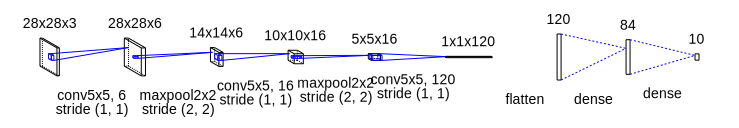
\includegraphics[width=15cm]{LeNet.png}
    \caption{LeNet}
\end{figure}
看到网上很多博客的解读,大部分会有3层卷积,也就是将我们这个lenet的第一个全连接层改为卷积。最开始我写的网络结构也是如此,但是发现在做grad\_cam的时候遇到了麻烦,
若是三层卷积,最后的卷积结果直接变成120*1*1,grad\_cam难以进行下去。后来,我发现,最后一层卷积和全连接的性质是一样的,二者参数量也是一样,120*16*5*5+bias。
于是,我将其改成了现在的这个结构,这样一来,grad\_cam也能正常进行了。

该神经网络作图开源:\href{https://alexlenail.me/NN-SVG/LeNet.html}{NN-SVG}\\
其余在本次实验过程中,找到的使我对CNN理解更生动、透彻的网页:\\
\href{https://poloclub.github.io/cnn-explainer/}{CNN explainer},\href{https://www.ruder.io/}{机器学习有意思的讲解}

\section{问题引入}
初级阶段,在三种训练环境中,数据分别为红色数字黑色背景、绿色数字黑色背景、白色数字黑色背景,在测试阶段,数据分别为黄色数字白色背景、蓝色数字白色背景。
\begin{figure}[H]
    \centering
    \includegraphics[width=12cm]{basic_train.png}
    \caption{Basic train}
\end{figure}
发现,即使在train1、train2、train3上的平均正确率已经达到一个较高值,在test1、test2上测试出来的正确率却很低,10\%左右,跟乱猜差不多。
\begin{figure}[H]  
    \begin{minipage}[H]{0.5\linewidth} % 图片占一行宽度0.5
            \centering
            \includegraphics[width=7.5cm]{basic_test1.png}
            \caption{Basic test1}
     \end{minipage}
     \begin{minipage}[H]{0.5\linewidth} %图片占用一行宽度的50%
         \hspace{2mm}%微调2mm
         \includegraphics[width=7.5cm]{basic_test2.png}
         \caption{Basic test2}
      \end{minipage}
\end{figure}
由此,我们对OOD现象有了一个初步的认识,分别在不同的字体颜色和背景颜色的组合下训练和测试,测试结果总是会很低,其实也就是该模型的泛化性很差,受背景等spurious feature的影响较大.

混淆矩阵作图参考:\href{https://blog.csdn.net/ZhangYuq16/article/details/97960165}{混淆矩阵\_CSDN}

\section{数据增广}
为应对模型泛化性差的问题,我们采取对数据进行增广的策略,保证模型“见过”颜色组合尽可能多的数据。
对此,我们对数据进行了第一次增广(主要由队友余俊洁负责各种颜色组合数据的调节和生成),
并将得到所有数据综合之前的train1、train2、train3得到data-12,并将其shuffle,并取3:1的训练验证占比,结果如下:
\begin{figure}[H]
    \centering
    \includegraphics[width=10cm]{train_on_12.png}
    \caption{Train on data-12}
\end{figure}
\begin{figure}[H]
    \centering
    \includegraphics[width=10cm]{val_on_12.png}
    \caption{Validation on data-12}
\end{figure}
\begin{figure}[H]  
    \begin{minipage}[H]{0.5\linewidth} % 图片占一行宽度0.5
            \centering
            \includegraphics[width=7.5cm]{test1_on_12.png}
            \caption{Test1}
     \end{minipage}
     \begin{minipage}[H]{0.5\linewidth} %图片占用一行宽度的50%
         \hspace{2mm}%微调2mm
         \includegraphics[width=7.5cm]{test2_on_12.png}
         \caption{Test2}
      \end{minipage}
\end{figure}
在训练该模型时,最开始,我取初始学习率为0.001,并加入学习率优化器,改变步长取10,乘积因子取0.1,发现在epoch10附近acc会骤降再上升,后取gamma=0.8,便得到上面的结果,在train和validation上都达到了95\%以上的正确率,在test1、test2上都有90\%左右的正确率。
可见,在进行了数据增广(模型并未“见过”test1、test2)之后,模型的泛化性得到了不少提升,由此得到model-12。

此外,队友还对数据添加了一些噪声,得到data-3,我们在model-12的基础上,在data3上取75\%的训练占比,再在test1、test2上测试,得到了model-3,结果如下:
\begin{figure}[H]  
    \begin{minipage}[H]{0.5\linewidth} % 图片占一行宽度0.5
            \centering
            \includegraphics[width=7.5cm]{acc_on_3.png}
            \caption{Train on data3}
     \end{minipage}
     \begin{minipage}[H]{0.5\linewidth} %图片占用一行宽度的50%
         \hspace{2mm}%微调2mm
         \includegraphics[width=7.5cm]{loss_on_3.png}
         \caption{Validation on data3}
      \end{minipage}
\end{figure}

\begin{figure}[H]  
    \begin{minipage}[H]{0.5\linewidth} % 图片占一行宽度0.5
            \centering
            \includegraphics[width=7.5cm]{test1_on_3.png}
            \caption{Test1}
     \end{minipage}
     \begin{minipage}[H]{0.5\linewidth} %图片占用一行宽度的50%
         \hspace{2mm}%微调2mm
         \includegraphics[width=7.5cm]{test2_on_3.png}
         \caption{Test2}
      \end{minipage}
\end{figure}
发现,经过data-3训练后,在test1、test2上的正确率提高到了95\%以上。



\section{可视化分析}
\subsection{参数敏感性及参数敏感性分析}
在该分析中,我关闭了学习率优化器,分别选取学习率为\[0.0001,0.0005,0.0008,0.001,0.003\]epoch为\[1\~15\]在data-12上训练和验证\(3:1\)(各组取同样的随机数种子来shuffle数据),
结果如下:
在训练集上:
\begin{figure}[H]  
    \begin{minipage}[H]{0.5\linewidth} % 图片占一行宽度0.5
            \centering
            \includegraphics[width=7.5cm]{acc_ana_train.png}
            \caption{Train acc on data-12}
     \end{minipage}
     \begin{minipage}[H]{0.5\linewidth} %图片占用一行宽度的50%
         \hspace{2mm}%微调2mm
         \includegraphics[width=7.5cm]{loss_ana_train.png}
         \caption{Train loss on data-12}
      \end{minipage}
\end{figure}
在验证集上:
\begin{figure}[H]  
    \begin{minipage}[H]{0.5\linewidth} % 图片占一行宽度0.5
            \centering
            \includegraphics[width=7.5cm]{acc_ana_val.png}
            \caption{Validation acc on data-12}
     \end{minipage}
     \begin{minipage}[H]{0.5\linewidth} %图片占用一行宽度的50%
         \hspace{2mm}%微调2mm
         \includegraphics[width=7.5cm]{loss_ana_val.png}
         \caption{Validation loss on data-12}
      \end{minipage}
\end{figure}
test1、test2上的平均acc和loss
\begin{figure}[H]  
    \begin{minipage}[H]{0.5\linewidth} % 图片占一行宽度0.5
            \centering
            \includegraphics[width=7.5cm]{acc_ana_test.png}
            \caption{Test acc on data-12}
     \end{minipage}
     \begin{minipage}[H]{0.5\linewidth} %图片占用一行宽度的50%
         \hspace{2mm}%微调2mm
         \includegraphics[width=7.5cm]{loss_ana_test.png}
         \caption{Test loss on data-12}
      \end{minipage}
\end{figure}


可见,当学习率较小时,结果的变化幅度较小,当学习率过大时,又容易导致波动过大,取0.001较为合适。
关于epoch,仍是取15合适。

\subsection{特征图可视化}
原图如下(本人手写):
\begin{figure}[H]
    \centering
    \includegraphics[width=5cm]{test_3.jpg}
    \caption{figure-3}
\end{figure}
第一次卷积和激活后的特征图:
\begin{figure}[H]  
    \begin{minipage}[H]{0.5\linewidth} % 图片占一行宽度0.5
            \centering
            \includegraphics[width=6cm]{f1_conv1_viridis.png}
            \caption{Convolution 1}
     \end{minipage}
     \begin{minipage}[H]{0.5\linewidth} %图片占用一行宽度的50%
         \hspace{2mm}%微调2mm
         \includegraphics[width=6cm]{f1_act1_viridis.png}
         \caption{Activate 1}
      \end{minipage}
\end{figure}
第一次池化和第二次卷积后的特征图:
\begin{figure}[H]  
    \begin{minipage}[H]{0.5\linewidth} % 图片占一行宽度0.5
            \centering
            \includegraphics[width=6cm]{f1_pooling1_viridis.png}
            \caption{Maxpooling 1}
     \end{minipage}
     \begin{minipage}[H]{0.5\linewidth} %图片占用一行宽度的50%
         \hspace{2mm}%微调2mm
         \includegraphics[width=6cm]{f1_conv2_viridis.png}
         \caption{Convolution 2}
      \end{minipage}
\end{figure}
第二次激活和池化后的特征图:
\begin{figure}[H]  
    \begin{minipage}[H]{0.5\linewidth} % 图片占一行宽度0.5
            \centering
            \includegraphics[width=6cm]{f1_act2_viridis.png}
            \caption{Activate 2}
     \end{minipage}
     \begin{minipage}[H]{0.5\linewidth} %图片占用一行宽度的50%
         \hspace{2mm}%微调2mm
         \includegraphics[width=6cm]{f1_pooling2_viridis.png}
         \caption{Maxpooling 2}
      \end{minipage}
\end{figure}

特征图及卷积核作图格式参考:Larry同学(哔哩哔哩)

\href{https://www.bilibili.com/video/BV17i421U73P?vd_source=c14e6c30a308a6303f3a1b9c65140798}{Larry同学bilibili}

\subsection{卷积核可视化}
\begin{figure}[H]  
    \begin{minipage}[H]{0.5\linewidth} % 图片占一行宽度0.5
            \centering
            \includegraphics[width=7cm]{kernel1.png}
            \caption{Kernel 1}
     \end{minipage}
     \begin{minipage}[H]{0.5\linewidth} %图片占用一行宽度的50%
         \hspace{2mm}%微调2mm
         \includegraphics[width=7cm]{f1_pooling2_viridis.png}
         \caption{Kernel 2}
      \end{minipage}
\end{figure}


\subsection{注意力分析(grad\_cam)}
原图如下(本人手写):
\begin{figure}[H]
    \centering
    \includegraphics[width=7cm]{test_9.jpg}
    \caption{figure-9}
\end{figure}
取用model-3,将目标层定为第二个卷积层,得到的热力图:
\begin{figure}[H]
    \centering
    \includegraphics[width=10cm]{focus_9.png}
    \caption{grad\_cam on figure-9}
\end{figure}

发现,该模型基本能将主要注意力放在数字9的关键部位,但也有不少注意力分散到了背景上。

Grad\_cam作图参考:
\href{https://arxiv.org/pdf/1610.02391v1}{paper}

\href{https://blog.csdn.net/qq_24211837/article/details/134263849}{pytorch\_grad\_cam的用法\_CSDN}

\section{IRM}

在该模块中,最初我看了一下关于IRM的论文及诸多阅读笔记(具体网址贴在下面),然后我的思路是在模型的输出中添加上预测环境标签的一项,对该标签的预测以及真实数字标签的预测的损失进行正则化,再去做Gradient Desent,
但是,跑了很多次,结果都不理想。环境预测损失项的系数$\lambda$若是太小,容易受环境的影响,若是过大,真实标签预测的正确率又会过低。
后来,我在GitHub上找到了一份开源的MNIST二分类的IRM实现,该博主对比了IRM和ERM两种思路下的训练和测试正确率,其中,博主使用了放缩过后的IRMv1,个人觉得很厉害的是,其中关于环境的penalty会随epoch来改变(系数 = 1.6*epoch),这个问题在那篇知乎中有提及,减小了overfitting的风险。

在本地,我将源代码中的网络结构改成了LeNet二分类的形式,对最终结果作图分析,得到的结果如下:
\begin{figure}[H]  
    \begin{minipage}[H]{0.5\linewidth} % 图片占一行宽度0.5
            \centering
            \includegraphics[width=7.5cm]{ERM.png}
            \caption{ERM}
     \end{minipage}
     \begin{minipage}[H]{0.5\linewidth} %图片占用一行宽度的50%
         \hspace{2mm}%微调2mm
         \includegraphics[width=7.5cm]{IRM}
         \caption{IRM}
      \end{minipage}
\end{figure}
发现,采用IRM的算法,加了关于环境的惩罚项之后,在源码中的train1、train2上训练,在test上较ERM的正确率提高了不少。

\href{https://github.com/reiinakano/invariant-risk-minimization}{我本地下的源码},\href{https://github.com/facebookresearch/InvariantRiskMinimization/tree/main}{源码博主推荐的official},
\href{https://briefgpt.xyz/kw/invariant20risk20minimization}{IRM相关的论文},\href{https://zhuanlan.zhihu.com/p/567666715}{IRM相关研究\_知乎},
\href{https://arxiv.org/abs/1907.02893}{paper},\href{https://paperswithcode.com/paper/invariant-risk-minimization}{paper with code}

\section{实验总结}
\begin{enumerate}
    \item 通过本次实验,我基本了解了OOD问题及其常见的解决方式
    \item 通过本次实验,我基本掌握了深度学习中的一些基本技巧,如模型基础训练、可视化分析等
    \item 通过本次实验,我对将来更深入的学习和研究激发了浓厚的兴趣,更有志于向前沿科研看齐
    \item 通过本次实验,我认识到在将来的工作中,与队友合作的重要性
\end{enumerate}

\end{document}
